\documentclass[conference]{IEEEtran}
\usepackage[T1]{fontenc}
\usepackage[utf8]{inputenc}
\usepackage{graphicx}
\usepackage{cite}
\usepackage{amsmath,amssymb}
\usepackage{booktabs}
\usepackage{array}
\usepackage{hyperref}
\usepackage{xcolor}
\usepackage{url}
\graphicspath{{./}}
\emergencystretch=2em
\hypersetup{colorlinks=true,linkcolor=black,citecolor=black,urlcolor=blue}
% Tighter spacing around floats (2-page demo limit)
\setlength{\textfloatsep}{6pt plus 2pt minus 2pt}
\setlength{\floatsep}{5pt plus 2pt minus 2pt}
% Never break these names across lines
\hyphenation{CAMARA OpenCAPIF UERANSIM AsSessionWithQoS}

\title{(DEMO) From Natural Language to Live 5G API Calls:
A CAPIF-Compliant, Multi-LLM Intent Orchestration Platform}
\author{
  \IEEEauthorblockN{T\"{u}rkan Do\u{g}a Durak$^{\ast}$,\; Engin Zeydan$^{\ddag}$,\; Luis Blanco$^{\ddag}$}\\
  \IEEEauthorblockA{%
    $^{\ast}$Universitat Polit\`{e}cnica de Catalunya (UPC), Barcelona, Spain.\\
    $^{\ddag}$Centre Tecnol\`{o}gic de Telecomunicacions de Catalunya (CTTC/CERCA), Castelldefels, Spain, 08860.\\
    Email: turkan.doga.durak@estudiantat.upc.edu,\; \{ezeydan, luis.blanco\}@cttc.es}
}

\begin{document}
\maketitle

\begin{abstract}
We demonstrate an open-source platform that converts free-text operator intents into
live CAMARA API calls. A two-phase large-language-model (LLM) planner selects the CAMARA
service and builds a schema-grounded payload, and a three-layer deterministic validator
(schema, telecom semantics, live CAPIF registry) gates every call. Quality of Service
(QoS) requests are authorized by the PCF of a containerized Open5GS 5G core with
UERANSIM-emulated UEs. A live request takes 2.2--4.8\,s with GPT-4o-mini or
Claude\,Haiku\,4.5 (6.9--8.2\,s with Gemini), 78--99\% of it LLM planning. On 300 unique
bilingual intents, the LLM planners reach an Intent-to-API Workflow Success Rate (IWSR)
of 95.3--97.3\%, versus 83.3\% for a keyword baseline and 16.3\% without schema grounding.
Code, testbed and data: \url{https://github.com/doadurak/mini-telco-platform}.
\end{abstract}

\begin{IEEEkeywords}
CAPIF, CAMARA, intent-based networking, LLM orchestration, 5G API exposure, Open5GS
\end{IEEEkeywords}

\section{Introduction}
Zero-touch Beyond-5G management requires orchestration layers that translate high-level
intents into standards-compliant API invocations~\cite{coronado2022}. 3GPP
CAPIF~\cite{3gpp_capif} and GSMA CAMARA~\cite{camara2022} standardize how verticals
discover and consume network capabilities, but closing the intent-to-API gap on a
\emph{live} exposure stack remains open. OpenCAPIF~\cite{molina2022} provides exposure
infrastructure without NL planning; Turkovic~et~al.~\cite{turkovic2025} ran live CAMARA
QoD with hand-written payloads; Maatouk~et~al.~\cite{maatouk2025} identify hallucination
as the key risk of telecom LLMs, and Liu~et~al.~\cite{liu2024} report 40\% JSON-schema
compliance for ungrounded GPT-4. Our platform combines live CAPIF onboarding,
schema-grounded multi-LLM planning, a three-layer validator, and CAMARA execution down
to a 3GPP PCF, reproducible from a single script.

\section{Platform Architecture}
\label{sec:arch}
\begin{figure}[t]
  \centering
  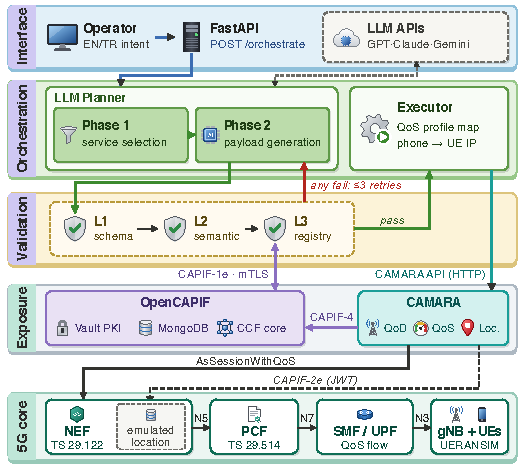
\includegraphics[width=\columnwidth]{fig1_architecture.pdf}
  \caption{Platform architecture. Any L1--L3 failure triggers at most three payload
  corrections; CAPIF-1e runs over mTLS, provider calls over HTTP.}
  \label{fig:arch}
\end{figure}
\textit{Planning:} A FastAPI backend exposes \texttt{POST\,/orchestrate}
(Fig.~\ref{fig:arch}). Phase\,1 selects one of four CAMARA services (QoD\,v1.1,
QoS\,Profiles, QoS\,Provisioning, Location\,Retrieval\,v0.5) from a schema-grounded
catalog; Phase\,2 populates the payload with the operation's OpenAPI schema
injected~\cite{flowmind2023}. Intent-level QoS classes (e.g.\
\texttt{QOS\_E\_STREAMING}) are mapped by target bit rate to the operator profiles the
network enforces (\texttt{QOS\_E/S/M/L}).

\textit{Validation:} L1 checks the payload against its Pydantic schema (pass rate: Schema
Compliance Rate, SCR). L2 enforces telecom rules (E.164 numbers, QoS profiles that map to
an operator profile, durations of 1--7200\,s, unicast IPv4); its pass rate is the
Semantic Validity Rate (SVR). L3 queries the live CAPIF registry to confirm that the
selected service is published; a wrong-but-registered service passes and shows up as an
IWSR miss against ground truth.

\textit{Execution:} For QoS, the adapter resolves the phone number to the UE's IP from
the 5GC subscriber database; the CAMARA provider forwards an AsSessionWithQoS
subscription to the NEF, which creates a PCF application session bound to the UE's PDU
session. Location uses the NEF Monitoring Event API with emulated core data.

\section{Live Demonstration}
\label{sec:demo}
\begin{figure}[t]
  \centering
  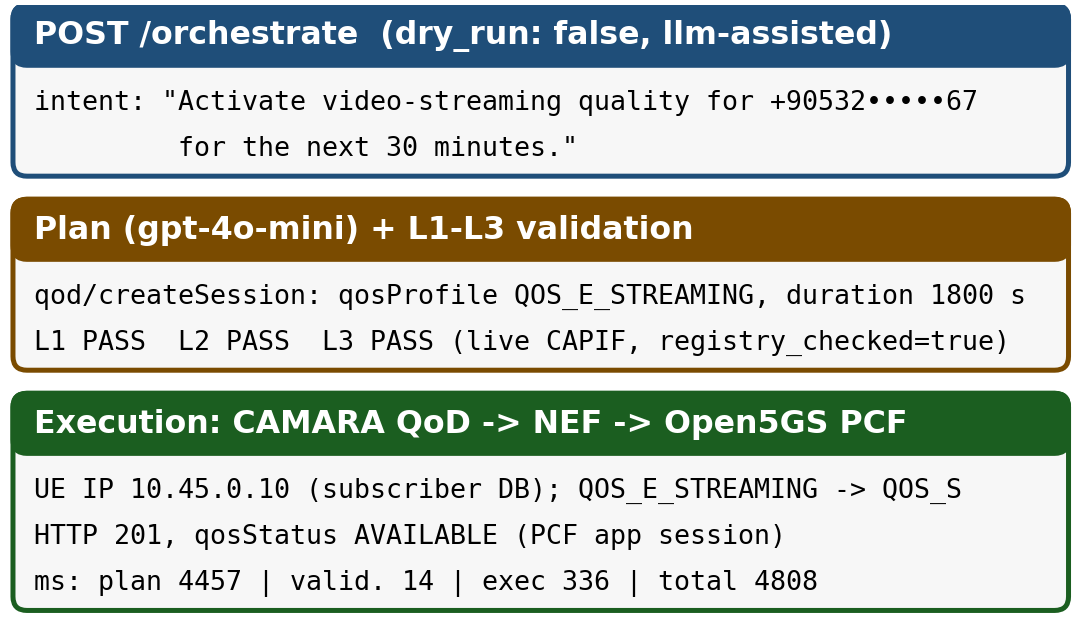
\includegraphics[width=0.85\columnwidth]{fig2_live_orchestrate.png}
  \caption{Recorded live response (S1, GPT-4o-mini, \texttt{dry\_run:false}), rendered
  from the stored JSON in the repository (MSISDN masked).}
  \label{fig:ui}
\end{figure}
The full stack (OpenCAPIF, four CAMARA/NEF providers, Open5GS, a UERANSIM gNB with three
UEs) runs on one 16\,GB host via \texttt{start.sh}; all scenarios run with
\texttt{dry\_run:false} and are versioned in the repository.
\textbf{S1 (QoD):} \textit{``Activate video-streaming quality for $\langle$MSISDN$\rangle$
for the next 30 minutes''} yields \texttt{QOS\_E\_STREAMING}, 1800\,s, enforced as
\texttt{QOS\_S}; the PCF accepts the session and QoD returns HTTP\,201,
\texttt{AVAILABLE} (Fig.~\ref{fig:ui}).
\textbf{S2 (Location):} the NEF returns a WGS-84 area (HTTP\,200).
\textbf{S3 (ambiguity):} dataset entry \textit{``Provide network quality improvement for
device $\langle$MSISDN$\rangle$ for a long time''} (ground truth: QoD). In the benchmark
GPT-4o-mini chose QoD and Claude and Gemini QoS\,Provisioning; live, all three chose
QoS\,Provisioning (PCF: \texttt{ACTIVE}). Every plan passes L1--L3 and executes: the
validator guarantees well-formed, registered calls, not intent correctness.
\textbf{S4 (backend switch):} after each \texttt{POST\,/config/provider} switch, S1
yields identical CAMARA payloads from all three LLMs. Validation takes 13--27\,ms and
execution 0.03--0.6\,s. UERANSIM lacks NGAP PDU Session Resource Modify, so the
dedicated QoS flow is authorized by the core but not enforced on the emulated radio.
\textit{Scalability and LLM APIs:} with the keyword planner and live L3, one backend
process sustains $\approx$160\,req/s (p95 156\,ms, 20 concurrent clients); with
GPT-4o-mini, latency stays at $\approx$2.6\,s up to 10 concurrent requests while
throughput grows linearly (0.34 to 3.3\,req/s): the LLM API, not the platform, is the
bottleneck. In \texttt{auto} mode an LLM error falls back to the keyword planner; since
intents (with MSISDNs) leave the testbed, production use needs pseudonymization or a
self-hosted model.

\section{Evaluation}
\begin{table}[t]
\centering
\caption{300-entry offline evaluation (one run per intent)}
\label{tab:metrics}
\footnotesize
\setlength{\tabcolsep}{2.6pt}
\begin{tabular}{lrrrrr}
\toprule
\textbf{Planner} & \textbf{IWSR} & \textbf{SCR} & \textbf{SVR} & \textbf{HR} & \textbf{SS} \\
\midrule
Keyword baseline   & 83.3\% & 100.0\% & 100.0\% & 16.7\% & 0.962 \\
GPT-4o-mini        & \textbf{97.3\%} & 100.0\% & 99.0\% & \textbf{2.3\%} & \textbf{0.975} \\
Claude\,Haiku\,4.5 & 95.3\% & 99.3\% & \textbf{99.3\%} & 4.0\% & 0.927 \\
Gemini\,2.5\,Flash & 96.0\% & 100.0\% & 98.3\% & 3.0\% & 0.945 \\
\midrule
\multicolumn{6}{l}{\textit{Ablations (GPT-4o-mini, no feedback loop)}} \\
Single LLM call    & 77.3\% & 78.0\% & 77.3\% & 3.3\% & 0.949 \\
No schema in Ph.\,2 & 16.3\% & 16.7\% & 16.7\% & 4.0\% & 0.947 \\
\bottomrule
\end{tabular}
\end{table}
\begin{table}[t]
\centering
\caption{Fault injection into correct GPT-4o-mini plans (live L3)}
\label{tab:faults}
\footnotesize
\setlength{\tabcolsep}{2.6pt}
\begin{tabular}{llrrr}
\toprule
\textbf{Layer} & \textbf{Injected fault} & \textbf{Caught} & \textbf{Repaired} & \textbf{Feedback} \\
\midrule
L1 & missing field, wrong type & 40/40 & 40/40 & 1.3\,s (1 it.) \\
L2 & E.164, duration, profile, IPv4 & 80/80 & 79/80 & 1.3\,s (1 it.) \\
L3 & service not published & 20/20 & 0/20 & 3.8\,s (3 it.) \\
\bottomrule
\end{tabular}
\end{table}
The dataset holds 300 unique intents (152\,EN / 148\,TR; 96 easy, 94 medium, 110 hard):
275 across the four services and 25 ambiguous edge cases. We derived the ground truth
(service, operation, payload checks) from the CAMARA OpenAPI constraints and NEF test
fixtures; it supersedes a 60-entry pilot (\texttt{datasets/legacy\_pilot\_60/}).%
\footnote{The first 60 LLM results per model are reused from the pilot; the Claude pilot
predates three bug fixes, and a symptom scan found no affected entry. Eleven multi-intent
entries were re-run after adding multi-step plans (flagged in the result files).}
IWSR counts plans with the correct service that pass validation; HR is the share of
wrong service selections; SS is $1-\sigma$ of IWSR across difficulty strata, not
run-to-run repeatability (temperature 0.1, so ambiguous choices can vary, cf.\ S3). The
benchmark makes no provider calls; all 1,200 recorded plans pass the live L3 check.
The keyword rules were written against the pilot (baseline 100\%); on the 240 held-out
entries the baseline drops to 79.2\% and the LLMs reach 95.4--97.1\%. LLM failures (8--14
per model) are mostly QoD vs.\ QoS Provisioning confusions as in S3; hard IWSR is
87--95\% vs.\ 99--100\% for easy and medium.
\textit{Ablations:} without the operation's schema and field rules in Phase\,2,
GPT-4o-mini invents field names and SCR falls to 16.7\% (cf.\ 40\% for ungrounded GPT-4
in~\cite{liu2024}); a single-call planner reaches 77.3\%, versus 96.7\% for our two-phase
planner without feedback.
\textit{Fault injection} (Table~\ref{tab:faults}): each fault is caught by its target
layer; feedback repairs L1/L2 faults in one iteration but cannot fix an unpublished or
wrong-but-registered service, since it only rewrites the payload.

{\footnotesize
\bibliographystyle{IEEEtran}
\bibliography{references_wmnc}
}
\end{document}
